\section{Klassische Enterprise-Architektur}

%%%%%%%%%%%%%%%%%%%%%%%%%% Monolith Architecture %%%%%%%%%%%%%%%%%%%%%%%%%%%



\begin{frame}{Monolith Architecture}
    \item Früher: Einstiegsarchitektur für viele große Unternehmen wie Netflix
    \item Komponenten sind in einem einzigen Code-Basis
    \item Besonders geeignet für kleine Anwendungen
\end{frame}



\begin{frame}{Monolith Architecture: Beispiel E-Commerce I}
    \begin{figure}[!h]
        \centering
        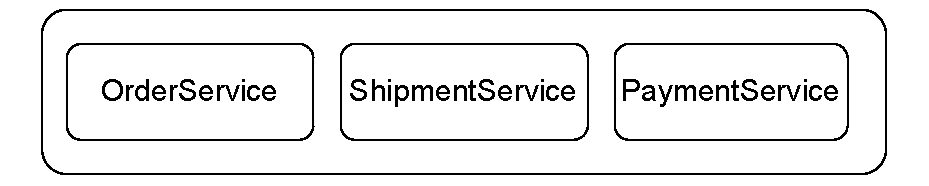
\includegraphics[scale=0.70]{imglib/mono/mono}
        \caption{E-Commerce-Beispiel mit Monolith Architektur}
        \label{fig:mono-ecommerce}
    \end{figure}
\end{frame}

\begin{frame}{Monotlith Architecture: Agilität}
    \begin{itemize}
        \item Mit zunehmender Komplexität und des Code-Bases wird die Skalierung und Wartung schwieriger
        \item Eng gekoppelte Komponenten verhindern die Wiederverwendung
        \item Autonome Teams können nicht unabhängig voneinander einzelne Komponenten entwickeln
        \item Änderungen an einer Komponente wirken sich auf andere Komponenten aus, was die Software-Lieferung verlangsamt
    \end{itemize}
\end{frame}

%%%%%%%%%%%%%%%%%%%%%%%%%% Modular Monolith Architecture %%%%%%%%%%%%%%%%%%%%%%%%%%%

\begin{frame}{Modular Monolith Architecture}
    \begin{itemize}
       \item Bisher: Eng gekoppelte Komponenten mit gegenseitigen Abhängigkeiten
       \item Jetzt: Module minimal gekoppelt und durch klare Schnittstellen definiert
       \item Alternative zur monolithischen Architektur, um die Abhängigkeiten zu reduzieren
       \item Abhängigkeiten bestehen weiterhin, müssen jedoch vom Entwickler auf ein Minimum reduziert werden
     \end{itemize}
\end{frame}

\begin{frame}{Monolith Architecture: Beispiel E-Commerce II}
    \begin{figure}[!h]
        \centering
        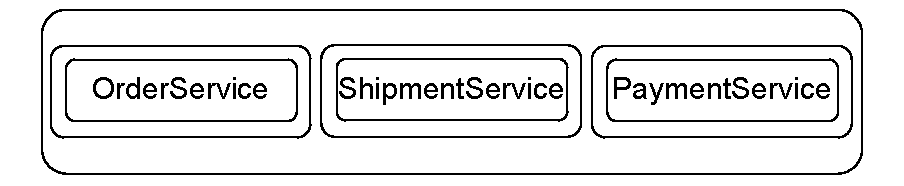
\includegraphics[scale=0.70]{imglib/mono/mono-example}
        \caption{Aufbau einer Modular monolitische Architektur}
        \label{fig:mono-modular}
    \end{figure}
\end{frame}

\begin{frame}{Modular Monolith Architecture: Agilität}
    \begin{itemize}
      \item Da Module miteinander verbunden sind, ist die Skalierung von einzelnen Modulen schwierig
      \item Abhängigkeiten zwischen Module verhindern weiterhin die parallele Entwicklung von Modulen
      \item Fehler in einem Modul können die Verfügbarkeit des gesamten System beeinträchtigen
    \end{itemize}
\end{frame}
